\documentclass[language=german,style=solution]{smo}

\examplace{Zürich}
\examdate{12./13./26./27. Mai 2018}

\title{SMO-Selektion - Musterlösung}

\begin{document}

\begin{enumerate}

\item[\textbf{1.}] %% Exercise 1 %%
Sei $k \geq 0$ eine ganze Zahl. Bestimme alle reellen Polynome $P$ von Grad $k$ mit $k$ verschiedenen reellen Nullstellen, sodass für alle Nullstellen $a$ von $P$ gilt:
\[
P(a+1) = 1.
\]

\textbf{Antwort:} Die Lösungen sind alle konstante Polynome $P(x) = c$ mit $c\neq 0$ und alle Polynome $P(x) = x+b$ mit $b\in\R$.

\textbf{Lösung 1:}
Alle konstanten Polynome \(P(x)=c\neq 0 \) sind Lösungen. Sei \(P\) nun ein solches Polynom mit Grad mindestens 1. Das Polynom \(Q(x)=P(x+1)-P(x)-1\) hat nach Vorraussetzung mindestens \(n\) verschiedene Nullstellen. Da \(Q\) aber maximal Grad \(n-1\) hat, folgt dass \(Q(x)=0\) bzw. \(P(x+1)=P(x)+1\) für alle \(x\in \mathbb{R}\) gilt. Daraus folgt, dass \(P\) Grad 1 hat, denn falls dem nicht so wäre, so würde ein Koeffizientenvergleich von \(x^{n-1}\) zu \(a_{n-1}+na_n=a_{n-1}\) führen (wobei \(P(x)=a_nx^n+a_{n-1}x^{n-1}+...+a_0 \)) und somit \(a_n=0\) implizieren, was natürlich nicht sein kann. Also hat $P$ Grad 1 und wir können $P(x) = ax + b$ schreiben. Sei $y$ seine Nullstelle. Nach Annahme gilt
\[
	1 = P(y+1) = a(y+1) + b = ay + b + a = P(y) + a = a.
\]
Also muss $a=1$ gelten. Für jede $b\in \R$ ist das Polynom $P(x) = x + b$ eine Lösung.

\textbf{Lösung 2:}
Sei $P(x) = c_k x^k + c_{k-1} x^{k-1}+...+c_0$. Wir wollen zuerst per widerspruch zeigen, dass $k<2$. (Wir bezeichnen die Nullstellen mit $a_1<\ldots<a_k$.)

Da $P(x)$ Grad $k$ hat, hat $P(x)$ auch höchstens $k$ einsstellen (weil $P(x)-1$ auch höchstens $k$ nullstellen hat). Da $P(a_i+1) = 1$ für alle nullstellen von $P$, müssen dies auch genau die einsstellen von $P$ sein.

Nehmen wir zuerst an, $k>1$ sei gerade. Dann muss der führende Koeffizient $c_k$ positiv oder negativ sein. Aber falls $c_k<0$ folgt dass $P(x)$ geht gegen $-\infty$ für $x$ gegen $\infty$, und dann muss $P(x) <0$ für alle $x > a_k$. Ein Widerspruch zu $P(a_k+1) = 1$.

Falls $c_k>0$ geht $P(x)$ gegen $\infty$ für $x$ gegen $-\infty$, und dann muss $P(x) = 1$ für ein $x < a_1$. Dies ist aber ein widerspruch zu $P(x)$ hat die einsstellen genau bei $P(a_i+1)$.

Wenn nun $k$ ungerade, dann kann man $P'(x) = P(x-a_1)$ nehmen. $P'$ sollte nun immernoch die Aufgabenstellung erfüllen und die kleinste Nullstelle ist $0$. Faktorisieren wir $P'(x) = x \cdot Q(x)$. Nun gilt für $Q(x)$ wieder, hat Grad $k-1$, hat $k-1$ verschieden nullstellen und $Q(a_i+1) > 0$. Dann, da $Q$ geraden Grad hat folgt mit der gleichen Fallunterscheidung wie oben ein Widerspruch.

Für den Grad < 2 lassen sich schnell die Lösungen finden.

\textbf{Solution 3:}
Si $k\geq 2$, soient $a_1<\ldots<a_k$ les zéros de $P$. On écrit $P(x)=c(x-a_1)\cdots(x-a_k)$. On sait que $P(a_k+1)=P(a_{k-1}+1)$. Donc
\begin{align*}
&(a_k-a_1+1)\cdots (a_k-a_{k-2}+1)(a_k-a_{k-1}+1)=\\
&(a_{k-1}-a_1+1)\cdots (a_{k-1}-a_{k-2}+1)(a_{k-1}-a_k+1).
\end{align*}
Or 
\begin{align*}
(a_k-a_1+1)&>(a_{k-1}-a_1+1),\\
&\ldots,\\
(a_k-a_{k-2}+1)&>(a_{k-1}-a_{k-2}+1),\\
(a_k-a_{k-1}+1)&>(a_{k-1}-a_k+1).
\end{align*}
C'est une contradiction, donc $k\leq 1$. On traite les cas $k=0,1$ comme dans la première solution

\textbf{Solution 4:}
Si $\deg(P)\geq 2$, soit $Q(x):=P(x)-1$ et $P(x)=a_kx^k+a_{k-1}x^{k-1}+\ldots + a_0$ avec zéros $x_1,\ldots,x_k$. Par les formules de Viète sur $P$ et sur $Q$, on a
\[
x_1+\ldots+x_k=-\frac{a_{k-1}}{a_k}= (x_1+1)+\ldots+(x_k+1)
\]
et donc $k=0$. Contradiction. On traite les cas $k=0,1$ comme dans la première solution.

\textbf{Marking scheme:}
\textit{Prouver que $k\leq 2$:} 5P.
\textit{Trouver les solutions avec $k\leq 1$:} +2P.

Pour la première étape, des points partiels peuvent être attribués de la manière suivante. Si plusieurs solutions ont été essayées, seule celle donnant le plus grand nombre de points est considérée:

\textbf{Solution 1:}
\begin{itemize}
\item introduire $Q$: 1P
\item $\deg(Q)\leq n-1$ ou $Q$ a $n$ racines: +1P
\item en déduire $Q\equiv 0$ et $P(x+1)=P(x)+1$: +2P
\end{itemize}


\textbf{Solution 2:}
\begin{itemize}
\item Beobachtung $P(x)$ hat genau $k$ einsstellen: 1P
\item Zeigen, dass $k$ nicht gerade sein kann: +2P
\item Faktorizierung von $P$ in ein Polynom mit Grad um eins kleiner: +1P
\end{itemize}

\textbf{Solution 3:}
\begin{itemize}
\item nommer les racines et factoriser $P(x)=c(x-a_1)\cdots(x-a_k)$: 0P
\item évaluer la factorisation en une racine $(a_i-a_1+1)\cdots (a_i-a_{k}+1)=1$: 1P
\item évaluer la factorisation en une \textbf{deuxième} racine $(a_i-a_1+1)\cdots (a_i-a_{k}+1)=(a_j-a_1+1)\cdots (a_j-a_{k}+1)$: 1P
\end{itemize}

\textbf{Solution 4:}
\begin{itemize}
\item Viète sur $P$: $x_1+\ldots+x_k=-\frac{a_{k-1}}{a_k}$: 2P
\item Viète sur $Q$: $(x_1+1) + \ldots + (x_k+1) = -\frac{a_{k-1}}{a_k}$: +1P
\end{itemize}

Pour les solutions incomplètes, on ne retire pas de point pour avoir oublié d'exclure $\deg(P)=0$ dans un argument. Dans toutes les solutions complètes, les points suivants sont retirés:
\begin{itemize}
\item les solutions constantes sont absentes: -1P
\item on ne mentionne pas que les solutions $P(x)=x+c$ sont vraiment solutions: -1P
\end{itemize}
\newpage

\item[\textbf{2.}] %% Exercise 2 %% 
Soit $ABC$ un triangle aigu et $O$ le centre de son cercle circonscrit. La droite $OA$ coupe la hauteur $h_b$ en $P$ et la hauteur $h_c$ en $Q$. Soit $H$ l'orthocentre du triangle $ABC$. Prouver que le centre du cercle circonscrit au triangle $PQH$ est sur la médiane du triangle $ABC$ passant par $A$.

\textit{Remarque: La hauteur $h_a$ est la droite perpendiculaire à $BC$ passant par $A$.}

%\begin{figure}[h!]
%	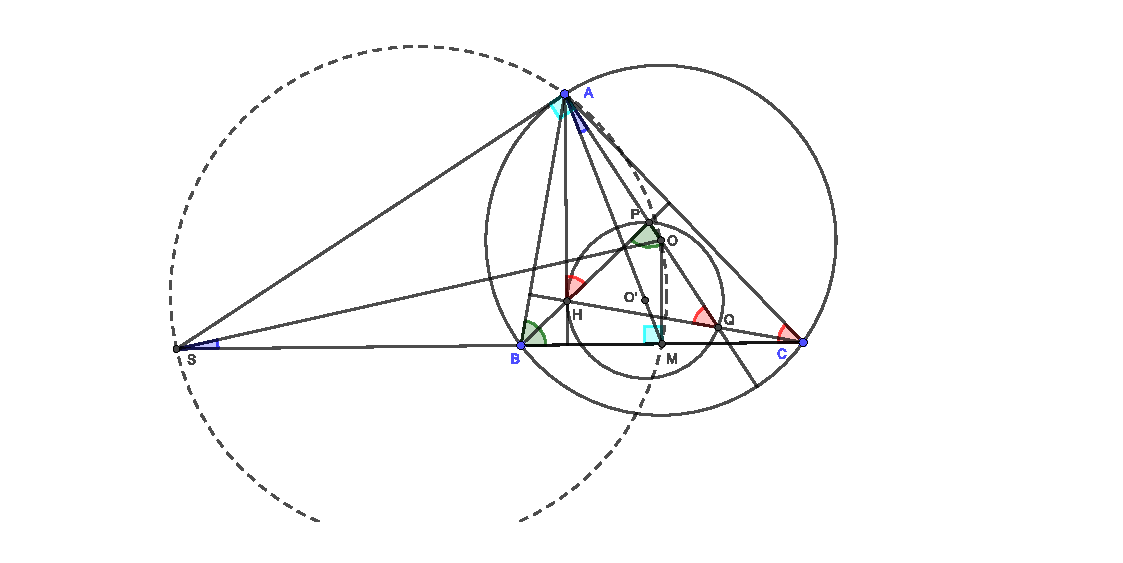
\includegraphics{imoselection_2018_Exercice2}
%\end{figure}

\textbf{Solution:}
On commence par une petite chasse aux angles. Soient $\alpha,\beta$ et $\gamma$ les trois angles du triangle $\Delta ABC$. Observez que $\angle HPQ=\pi/2-\angle PAC$ parce que $PH$ est perpendiculaire à $AC$. De plus, comme $OA$ est un diamètre du cercle circonscrit à $\Delta ABC$ on a $\beta=\pi/2-\angle OAC=\pi/2-\angle PAC$. Ainsi $\angle HPQ=\beta$ et de manière similaire $\angle PQH=\gamma$. On en déduit que $\Delta ABC\sim \Delta HPQ$. Par chasse aux angles, on obtient aussi que $\angle AHP =\gamma$ et donc $AH$ est la tangente au cercle circonscrit de $\Delta PQH$ en $H$.

L'idée est à présent d'introduire la tangente au cercle circonscrit à $ABC$ en $A$ par similarité avec le triangle $\Delta PQH$. Soit $t$ cette tangente et $S$ son intersection avec la droite $BC$. Si $O'$ est le centre du cercle circonscrit de $\Delta PQH$, alors la similarité de la construction implique que $\Delta AO'Q\sim \Delta SOC$.

Soit $M$ l'intersection de $AO'$ avec le coté $BC$. Comme $\angle O'AQ=\angle OSC$, on en déduit que $AOMS$ est un quadrilatère inscrit. Donc $\angle SMO=\pi-\angle SAO=\pi/2$. On conclut que $OM$ est perpendiculaire à $BC$ et donc $M$ est le milieu de $BC$.


\textbf{Marking scheme:}
\begin{enumerate}
\item chasse aux angles: total 2P
\begin{itemize}
\item explicitement obtenir $\Delta ABC\sim \Delta HPQ$: 1P 
\item $\angle PHA=\gamma$ et déduire que $AH$ est tangente: 1P
\end{itemize}
\item arguments par similarité: total 3P
\begin{itemize}
\item un argument par similarité (eg. introduire $t$, introduire $HO'$ et calculer des angles): 1P
\item conclure $\Delta AO'Q\sim \Delta SOC$ ou similaire: 2P
\end{itemize}
\item conclusion: 2P

Éléments ne valant aucun point:
\begin{itemize}
\item reformuler la conclusion de manière triviale (eg. $OM\perp BC$)
\item introduire la hauteur $h_a$
\item chasse aux angles sur un dessin
\end{itemize}

\end{enumerate}

\newpage

\item[\textbf{3.}] %% Exercise 3 %%
Entlang der Küste einer kreisrunden Insel befinden sich 20 verschiedene Dörfer. Jedes dieser Dörfer hat 20 Kämpfer, wobei alle 400 Kämpfer unterschiedlich stark sind.

Jeweils zwei benachbarte Dörfer $A$ und $B$ machen nun einen Wettkampf, indem sich jeder der 20 Kämpfer des Dorfs $A$ mit jedem der 20 Kämpfer des Dorfs $B$ misst. Dabei gewinnt jeweils der stärkere Kämpfer. Wir sagen, dass das Dorf $A$ \emph{stärker} ist als das Dorf $B$, falls in mindestens $k$ der 400 Kämpfe ein Kämpfer von Dorf $A$ gewinnt.

Es stellt sich heraus, dass jedes Dorf stärker als sein Nachbardorf im Uhrzeigersinn ist. Bestimme den maximalen Wert von $k$, sodass dies der Fall sein kann.

\textbf{Antwort:} Der maximale Wert ist $k= 290$.

\textbf{Lösung:}

Wir geben zuerst eine Konstruktion und beweisen dann, dass mehr als 290 nicht möglich ist. O.B.d.A können wir annehmen, dass die Kämpfer Stärken $1$ bis $400$ haben, und wir nummerieren die Dörfer im Uhrzeigersinn von eins bis zwanzig.

\textbf{Konstruktion:} Im ersten Dorf leben die Kämpfer der Stärke $400, 190, 189, 188, \ldots, 174,173,172$. Im zweiten Dorf leben $399,398,171,170,\ldots, 157,156$, und so weiter, im letzten Dorf leben die Kämpfer $210, 209, \ldots, 192,191$. Anschaulicher gesagt verteilen wir zuerst die Kämpfer mit Stärke grösser als 190 auf die Dörfer auf, ins erste Dorf 400, ins zweite Dorf 399, 398, ins dritte Dorf 397, 396, 395, usw. Dann füllen wir die Dörfer mit Kämpfer mit Stärke maximal 190 auf, ins erste Dorf $190,\ldots,172$, ins zweite Dorf $171,\ldots, 156$, usw.

Bemerke, dass Dorf $x$ gerade $x$ Kämpfer der Stärke grösser als 190 hat und $20-x$ Kämpfer der Stärke kleiner als 191. Für $x\in \{1,\ldots, 19\}$ gewinnen die Kämpfer mit Stärke grösser als 190 gegen alle Kämpfer des Dorfs $x+1$. Die Kämpfer der Stärke kleiner als 191 gewinnen gegen die Kämpfer der Stärke kleiner als 191 im nächsten Dorf, also gewinnen sie je $(20-(x+1))$ Mal. Insgesamt gewinnt Dorf $x$ also $20x+(20-x)(20-(x+1))$ Mal. Ausrechnen ergibt, dass jedes dieser Dörfer mindestens 290 Mal gewinnt. Nun betrachten wir noch das zwanzigste Dorf. Seine Kämpfer gewinnen gegen neunzehn Kämpfer vom Dorf eins, also gewinnt das zwanzigste Dorf mehr als 290 Mal. Somit ist $k=290$ möglich.

\textbf{Obere Schranke:} Nehme an, dass $k>290$ geht. Wir nennen Kämpfer mit Stärke maximal 200 \textit{schwach}. Es gibt 200 schwache Kämpfer und zwanzig Dörfer, also gibt es per Schubfachprinzip mindestens ein Dorf, das mindestens 10 schwache Kämpfer hat. Wir zählen, wie viel Mal dieses Dorf gewinnen kann. Die restlichen Kämpfer des Dorfs gewinnen insgesamt maximal $10\cdot 20=200$ Mal. Somit müssen die 10 schwachen Kämpfer mindestens 91 Mal gewinnen. Es folgt wiederum mit Schubfachprinzip, dass mindestens einer der 10  schwachen Kämpfer 10 Mal gewinnen muss. Folglich hat auch das nachfolgende Dorf mindestens 10 schwache Kämpfer. Mit dem gleichen Argument folgern wir reihum, dass jedes Dorf mindestens 10 schwache Kämpfer hat. Weiter folgt aus dem Argument, dass der stärkste der schwachen Kämpfer jeweils stärker sein muss als der stärkste der schwachen Kämpfer vom nachfolgenden Dorf, da er sonst nicht 10 Mal gewinnen kann. Daraus folgt aber auch, da wir das Argument reihum anwenden können, dass der stärkste der schwachen Kämpfer im ersten Dorf stärker sein muss als er selbst, was nicht möglich ist. Widerspruch, folglich ist $k\leq 290$.

\textbf{Marking Scheme:}
\begin{itemize}
	\item 3P Konstruktion, -1 falls 290 nicht richtig ausgerechnet
	\item 1P 10 schwache Kämpfer in einem Dorf, 11- oder 10-stärksten Kämpfer betrachten
	\item 1P 10 schwache Kämpfer im nächsten Dorf mit Stärkenungleichung, 11- oder 10- stärkster Kämpfer im nächsten Dorf ist schwächer
\end{itemize}


\newpage

\item[\textbf{4.}] %% Exercise 4 %%
Soit $n$ un nombre naturel pair. On partitionne les nombres $1, 2, \ldots, n^2$ en deux ensembles $A$ et $B$ de taille égale, de telle manière que chacun des $n^2$ nombres appartient à exactement un des deux ensembles. Soient $S_A$ et $S_B$ la somme de tous les éléments dans $A$ et $B$ respectivement. Déterminer tous les $n$ pour lesquels il existe une partition telle que
\[
\frac{S_A}{S_B} = \frac{39}{64}.
\]

\textbf{Réponse:}
Les nombres naturels $n$ recherchés sont tous les multiples de $206$.

\textbf{Solution:}
Soit $k$ le nombre entier tel que $S_A = 39k$ et $S_B = 64k$. On a alors que la somme de tous les nombres de $1$ à $n^2$ vaut
\[
	\frac{n^2(n^2+1)}{2} = S_A + S_B = 39k + 64k = 103k.
\]
Ainsi, $103 \div \frac{n^2(n^2+1)}{2}$, et comme $103$ est un nombre premier il doit diviser soit $\frac{n^2}{2}$, soit $n^2+1$. Cependant, puisque $n^2$ et $1 = 1^2$ sont premiers entre eux, tous les diviseurs premiers de $n^2+1$ doivent être congruents à $1 \mod 4$. Puisque $103 \equiv 3\mod 4$, il ne peut donc pas diviser $n^2+1$ et ainsi il doit être un diviseur de $\frac{n^2}{2}$. Cela ne peut être le cas que si $103 \div n$, donc puisque $n$ doit être pair il ne peut y avoir de solution que si $n$ est un multiple de $206$.

Montrons maintenant que, si $n = 206 m$ pour un certain nombre naturel $m$, il existe une telle partition. Dans ce cas on a
\[
	k = \frac{S_A+S_B}{103} = \frac{n^2(n^2+1)}{206}
\]
et il suffit de montrer que l'on peut choisir la moitié des nombres de sorte à ce que leur somme vaille $39k$. En effet, dans ce cas la somme des nombres restants vaudra nécessairement $64k$. Nous prouvons ici une propriété plus forte, à savoir que \emph{toutes} les sommes de $\frac{n^2(n^2+2)}{8}$ à $\frac{3n^4+2n^2}{8}$ sont atteignables. Puisque $\frac{n^2(n^2+2)}{8} = \frac{103k}{4} < 26k < 39k < \frac{103k}{2}$, cela termine la preuve. Les deux sommes extrêmes peuvent être obtenues en prenant respectivement tous les nombres de $1$ à $\frac{n^2}{2}$ et tous les nombres de $\frac{n^2}{2}+1$ à $n^2$. Maintenant si nous prenons une partition avec $S_A > \frac{n^2(n^2+2)}{8}$, l'ensemble $A$ doit contenir un nombre plus grand que $\frac{n^2}{2}$ et donc $B$ doit contenir un nombre plus petit ou égal à $\frac{n^2}{2}$. En particulier cela signifie qu'il existe un nombre dans $A$ qui est strictement plus grand qu'un nombre dans $B$. Il existe donc un nombre $x$ tel que $x\in B$ et $x+1\in A$. En échangeant $x$ et $x+1$, la somme dans $A$ diminue donc de $1$, ce qui prouve qu'il est effectivement possible d'atteindre toutes les sommes.

\textbf{Solution 2 (Yunshu):}
On prouve comme dans la première solution que $n$ doit être un multiple de $206$. Pour la construction, on va prouver par récurrence que pour tout $m\in \N$ il est possible de trouver un sous-ensemble $A$ de l'ensemble $\frack{1, 2, \ldots, 206m}$ contenant $103m$ éléments et tel que la somme des éléments de $A$ vaille
\[
	\frac{39}{103}\frac{206m(206m + 1)}{2} = 39m(206m + 1).
\]
L'ensemble $B$ est alors le complémentaire de $A$ et par construction on aura $\frac{S_A}{S_B} = \frac{39}{64}$. On va de plus prouver que le plus grand nombre dans $A$ ne dépasse pas $39*4m = 156m$

On commence avec $m=0$ et $A$ l'ensemble vide. Dans ce cas $S_A$ vaut trivialement $\frac{39}{103}$ fois la somme de tous les éléments entre $1$ et $206m$. Évidemment on ne peut pas calculer $\frac{S_A}{S_B}$ dans ce cas mais cela permet d'avoir un cas de base pour l'induction. Maintenant supposons que l'on ait construit un ensemble $A$ pour $m$ avec toutes les propriétés susmentionnées et construisons $A'$ pour $m+1$. On rajoute les nombres $1+206m, \ldots, 206 + 206m$, donc la somme totale augmente de
\[
	\frac{206*207}{2} + 206*206m = 103(207 + 103*4m)
\]
donc il faut rajouter 103 nombres à $A$ dont la somme vaut 
\[
	39(207 + 103*4m) = 102*39(4m+2) + 39(4m+3).
\]
Pour cela on rajoute à $A$ les 51 paires $(39(4m+2)-i, 39(4m+2)+i)$ avec $1\leq i\leq 52$ et $i\neq 39$ ainsi que le nombre $39(4m+2)+39 = 39(4m+3)$. Par construction ces 103 nombres donnent la somme voulue et comme $2*39 = 78 > 52$, le plus petit nombre rajouté est plus grand que $39*4m$ et le plus grand nombre rajouté est plus petit que $39(4m+4) = 39*4(m+1)$. Cela prouve que aucun des nombres rajoutés n'appartenait déjà à $A$ et que la condition sur le plus grand nombre de $A$ reste vérifiée. Finalement puisque nous avions commencé avec un ensemble $A$ qui était solution pour $m$, par construction le nouvel ensemble $A'$ est solution pour $m+1$.

\textbf{Marking scheme:}

\textit{Il n'existe pas de solution si $103\ndiv n$:} Total 4 Pt.
\begin{itemize}
	\item $103 \div \frac{n^2(n^2+1)}{2}$ : 1 Pt.
	\item $103 \ndiv n^2+1$ : +2 Pt.
	\begin{itemize}
		\item Idée de preuve pour $103 \ndiv n^2+1$ (p. ex. ordres ou résidus quadratiques): 1 Pt.
	\end{itemize}
	\item Il est nécessaire que $103 \div n$ : +1 Pt.
\end{itemize}

\textit{Il existe une solution si $103\div n$:} Total 3 Pt.
\begin{itemize}
	\item $S_A$ peut prendre n'importe quelle valeur entre $\frac{n^2(n^2+2)}{8}$ et $\frac{3n^4+2n^2}{8}$ : 2 Pt.
	\item $\frac{n^2(n^2+2)}{8} < 39k < \frac{3n^4+2n^2)}{8}$ : +1 Pt.
\end{itemize}

\newpage

\item[\textbf{5.}] %% Exercise 5 %%

Für eine natürliche Zahl $n$ sei ein $n \times n$ Brett gegeben. Wir färben nun $k$ der Felder schwarz ein, sodass es für jeweils drei Spalten maximal eine Reihe gibt, in der alle Kreuzungsfelder mit den drei Spalten schwarz gefärbt sind. Zeige, dass gilt:
\[
\frac{2k}{n} \leq \sqrt{8n-7}+1.
\]

\textbf{Lösung:}

Wir zählen für jedes Paar von Reihen die Anzahl Spalten, sodass beide Reihen in dieser Spalte schwarz sind.
Offensichtlich sind das höchstens 2 für jede der ${n \choose 2}$ Kombinationen, also insgesamt maximal $n(n-1)$. Wenn es in der i-ten Spalte also $a_i$ schwarze Quadrate sind, zählen wir jedes dieser Quadrate mindestens ${a_i \choose 2}$ mal. Wenn man nun über alle Spalten summiert, erhält man :

$\sum_{i=1}^{n} {a_i \choose 2} \leq n(n-1) \; \Leftrightarrow \ \sum_{i=1}^{n} \frac{a_i^2 - a_i}{2} \leq n(n-1) \; \Leftrightarrow \ \sum_{i=1}^{n} {a_i^2 - a_i} \leq 2n(n-1).$

Nun gilt $\sum_{i=1}^{n}{a_i} = k $ 
und mit CS, Chebychef oder ähnlichem:
$\sum_{i=1}^{n}{a_i^2} \geq \frac{(\sum_{i=1}^{n}{a_i})^2}{n} = \frac{k^2}{n}$ , also gilt $\frac{k^2}{n} - k \leq \sum_{i=1}^{n} {a_i^2 - a_i} \leq 2n(n-1) \; \Rightarrow \; k^2 - nk - 2n^2(n-1) \leq 0.$

Auf der LS steht ein quadratisches Polynom in k mit positivem Leitkoeffizient, insbesondere muss also k kleiner oder gleich der grösseren Nullstelle dieses Polynoms sein, dh:

$k \leq \frac{n + \sqrt{n^2 + 8n^2(n-1)}}{2} \; \Leftrightarrow \; \frac{2k}{n} \leq \sqrt{8n-7} + 1$


\textbf{Marking scheme:}
\begin{itemize}
    \item 2P : Die Formel $2*{n \choose 2}$ fnden.
    \item 3P : Die Formel $\sum_{i=1}^{n} \frac{a_i^2 - a_i}{2}$ finden.
    \item 2P : Den Beweis vollenden.
\end{itemize}

\newpage


\item[\textbf{6.}] %% Exercise 6 %%
Seien $A, B, C$ und $D$ vier Punkte, die in dieser Reihenfolge auf einem Kreis liegen. Nehme an, es gibt einen Punkt $K$ auf der Strecke $A$B, sodass $BD$ die Strecke $KC$ und $AC$ die Strecke $KD$
halbiert. Bestimme den kleinstmöglichen Wert, den $\left| \frac{AB}{CD}\right|$ annehmen kann.

\textbf{Réponse:} Le minimum est 2.

\textbf{Solution:}
\textit{On n'utilise que des distances non-orientées (i.e. positives).}

On obtient une construction si $ABCD$ est un trapèze isocèle avec base $AB=2CD$ et $K$ le milieu de $AB$.

La condition sur les milieux implique que $[ADC]=[AKC]$ où la notation crochets signifie l'aire du triangle. Si l'on pose $\alpha:=\angle CAD=\angle DBC$ et $\beta:=\angle BAC=\angle BDC$, on obtient
\begin{align*}
[ADC]&=\frac{1}{2}\sin (\alpha)\cdot AC\cdot AD\\
[AKC]&=\frac{1}{2}\sin (\beta)\cdot AC\cdot AK.
\end{align*}
Donc $AK/AD=\sin (\alpha)/\sin (\beta)$. Si on applique le théorème du sinus au triangle $\Delta BCD$, on obtient
\[
\frac{\sin (\alpha)}{\sin (\beta)}=\frac{CD}{BC}
\]
et donc $AK/CD=AD/BC$. Par symétrie, $BK/CD=BC/AD$. Finalement, avec AMGM:
\[
\frac{AB}{CD}=\frac{AK}{CD}+\frac{BK}{CD}=\frac{AD}{BC}+\frac{BC}{AD}\geq 2.
\]

\textbf{Solution (sans sinus):}
On introduit la projection orthogonale $H$ de $C$ sur $AD$ et la projection orthogonale $H'$ de $C$ sur $AB$. On a 
\begin{align*}
[ADC]&=AD\cdot CH\\
[AKC]&=AK\cdot CH'.
\end{align*}
De plus, $\Delta CHD\sim\Delta CH'B$ et donc $CH/CD=CH'/CB$. On obtient ainsi de même, $AK/CD=AD/BC$.




\textbf{Marking scheme:}
\begin{itemize}
\item $\left| \frac{AB}{CD}\right|\leq 2$ (construction): 2P
\item $\left| \frac{AB}{CD}\right|\geq 2$: 5P. 
\end{itemize}

Les points partiels suivants ne sont pas additifs:
\begin{itemize}
\item transformer la condition sur les milieux en une condition sur les aires: 2P
\item écrire $AK$ comme un ratio utile de distances ou d'angles
\item $AK/CD=AD/BC$ ou similaire: 4P
\end{itemize}



\newpage

\item[\textbf{7.}] %% Exercise 7 %%
Sei $n$ eine natürliche Zahl. Wir nennen eine Sequenz bestehend aus $3n$ Buchstaben \emph{rumänisch}, falls die Buchstaben $I$, $M$ und $O$ alle genau $n$ Mal vorkommen. Ein \emph{swap} ist eine Vertauschung von zwei benachbarten Buchstaben. Zeige, dass für jede rumänische Sequenz $X$ eine rumänische Sequenz $Y$ existiert, sodass mindestens $\frac{3n^2}{2}$ swaps nötig sind, um die Sequenz $Y$ aus der Sequenz $X$ zu erhalten.

\textbf{Lösung:}

Wir nummerieren die Positionen der Buchstaben von $1$ bis $3n$ und berechnen für jede Sorte von Buchstaben $\{I,M,O\}$ die Differenz zwischen der Summe ihrer Positionen und der Summe der Positionen $1, \dots , n$:
\[
S_I := \sum_{j=1}^n{p_j(I)} - \sum_{j=1}^n{j}
\]
\[
S_M := \sum_{j=1}^n{p_j(M)} - \sum_{j=1}^n{j}
\]
\[
S_O := \sum_{j=1}^n{p_j(O)} - \sum_{j=1}^n{j}
\]

wobei $p_j(I)$ die Position des $j$-ten Buchstabens $I$ in der Sequenz bezeichnet. Summieren wir die drei Gleichungen, erhalten wir:
\[
S_I+S_M+S_O \; = \; \sum_{j=1}^n{p_j(I)+p_j(M)+p_j(O)} \; - \; 3(\sum_{j=1}^n{j}) \; = \; \sum_{j=1}^{3n}{j} \; - \; 3(\sum_{j=1}^n{j}) \]
\[
= \; \frac{3n(3n+1)}{2} - 3\frac{n(n+1)}{2} \; = \; \frac{9n^2 + 3n - 3n^2 - 3n}{2} \; = \; 3n^2
\]

Also können nicht alle der Summen $S_I, S_M, S_O$ kleiner als $n^2$ sein. Sei am Anfang oBdA $S_I \geq n^2$. Da sich $S_I$ bei einem Swap höchstens um eins verringern kann, benötigen wir sicher mindestens $n^2$ Swaps, um alle $I$ nach ganz links zu bringen. Zudem gilt: Vertauschen wir ein $I$ mit einem benachbarten Buchstaben, ändert sich die relative Anordnung der $M$ und $O$ nicht, also können wir ein ähnliches Argument mit $M$ und $O$ durchführen:

Um die Lösung etwas abwechslungsreicher zu gestalten, zählen wir dieses Mal die Anzahl verschiedener Paare aus jeweils einem $M$ und $O$. Offensichtlich sind dies genau $n^2$. Unterscheiden wir nun die Anzahl Paare $P_1$, in denen $M$ links von $O$ steht und die Anzahl Paare $P_2$, in denen $M$ rechts von $O$ steht, folgt, dass es von einer Sorte mindestens $\frac{n^2}{2}$ geben muss. Sei am Anfang oBdA $P_2 \geq \frac{n^2}{2}$. Auch diese Grösse ändert sich pro Swap höchstens um 1 (und zwar genau dann, wenn wir ein $M$ mit einem $O$ vertauschen, also müssen wir, um alle $O$ nach ganz rechts zu bringen, noch mindestens $\frac{n^2}{2}$ Swaps durchführen.

Insgesamt gilt also: \; Um die Sequenz $I, \dots ,I,M, \dots, M,O, \dots ,O$ zu erhalten, benötigt man mindestens $n^2 + \frac{n^2}{2} = \frac{3n^2}{2}$ Swaps.
Diese dürfen wir zusammenzählen, weil die Swaps, die $S_I$ verringern, $P_2$ unverändert lassen und umgekehrt.

\textbf{Solution 2:}

On considère les deux suites $A = I\ldots IM \ldots MO \ldots O$ et $B = O\ldots OM \ldots MI \ldots I$. Pour passer d'une suite à l'autre, chaque paire de lettres différentes ($ (I, M), (I, O) et (M, O)$) doit être permutée au moins une fois. Puisqu'il existe $3n^2$ telles paires, il faut donc au minimum $3n^2$ swaps pour passer de la première suite à la seconde. Si l'on prend maintenant n'importe quelle suite $X$, on peut choisir $Y$ qui est soit $A$, soit $B$. En effet si ces deux suites pouvaient être obtenues depuis $X$ en strictement moins de $\frac{3n^2}{2}$ swaps, alors en passant par $X$ il serait possible d'aller de $A$ à $B$ en strictement moins de $3n^2$ swaps.

\textbf{Marking Scheme}

\textbf{Lösung 1:}
\begin{itemize}
\item +1P: Idee, die Buchstaben zu sortieren
\item +3P: Berechnung der Anzahl Swaps für eine Sorte Buchstaben
\item +2P: Berechnung für die zweite Sorte
\item +1P: fertig machen
\item $-$1P: Fehlende Argumentation, dass die verschiedenen Arten von Swaps disjunkt sind.
\end{itemize}

\textbf{Solution 2:}
\begin{itemize}
	\item 2P: Considérer les deux suites $A$, $B$ et la distance entre les deux.
	\item +3P: Prouver que la distance entre $A$ et $B$ vaut $3n^2$.
	\item 2P: Prouver l'exercice sous la supposition qu'il existe deux suites dont la distance vaut au minimum $3n^2$.
\end{itemize}

\newpage

\item[\textbf{8.}] %% Exercise 8 %%
Déterminer tous les nombres naturels $n\geq 2$ tels que pour tous les nombres entiers $0 \leq i,j \leq n$:
\[
i+j \equiv \binom{n}{i} + \binom{n}{j} \pmod{2}.
\]

\textbf{Réponse:} Les solutions sont tous les nombres de la forme $n = 2^k - 2$ avec $k\geq 2$.

\textbf{Solution:}

En posant $j = i+1$ (pour $i < n$), on obtient
\[
	\binom{n+1}{i+1} = \binom{n}{i} + \binom{n}{i+1} \equiv i + i + 1 \equiv 1 \pmod{2}.
\]
Ainsi, puisque $\binom{n+1}{0} = 1$, cela signifie que pour tout $0\leq i \leq n+1$ le nombre $\binom{n+1}{i}$ doit être impair. Pour tout $0\leq i\leq n+1$ on peut écrire
\[
	\binom{n+1}{i} = \frac{(n+1)\cdot n\cdot(n-1)\cdot\ldots\cdot (n+2-i)}{1\cdot 2\cdot\ldots\cdot i},
\]
donc puisque pour passer de $i-1$ à $i$ on multiplie par $q= \frac{n+2-i}{i}$ et que $\binom{n+1}{i-1}$ et $\binom{n+1}{i}$ sont tous les deux impairs, cela signifie que la fraction irréductible associée à $q$ doit être un quotient de deux nombres impairs. Autrement dit, il faut que pour tout $1\leq i\leq n+1$ les deux nombres $n+2-i$ et $i$ admettent le même nombre de facteurs $2$ dans leur décomposition en nombre premier.

On veut montrer que $n+2$ est une puissance de $2$. Soit $2^l$ la plus grande puissance de $2$ qui soit strictement inférieure à $n+2$. En particulier on a $2^l \geq \frac{n+2}{2}$. Considérons donc $i = 2^l$. Il faut alors que $2^l$ divise $n+2 - 2^l$, et comme $n+2 - 2^l \leq 2^l$, ce n'est le cas que si $n+2 = 2^{l+1}$.

Il reste à prouver que tous les nombres de la forme $n = 2^k-2$ sont effectivement solution. Pour cela il suffit en fait de prouver que $\binom{n}{i} \equiv i+1 \pmod{2}$ pour tout $0\leq i\leq n$. En effet si c'est le cas on a alors
\[
	\binom{n}{i} + \binom{n}{j} \equiv i + j + 2 \equiv i + j \pmod{2}.
\]
On va montrer cette propriété par induction sur $i$. Pour $i = 0$ et $i = 1$ on a clairement $\binom{n}{i}\equiv i + 1 \pmod{2}$. Supposons maintenant que la propriété a déjà été prouvée jusqu'à $i-1$. Si $i$ est impair, on multiplie le nombre précédent par $\frac{n+1-i}{i}$, et comme le numérateur est pair alors que le dénominateur est impair on a effectivement que $\binom{n}{i}$ est pair. Si $i$ est pair on multiplie $\binom{n}{i-2}$ par $\frac{n+1-i}{i-1}\cdot\frac{n+2-i}{i}$. La première fraction est un quotient de deux nombres impairs, et comme $n+2 = 2^k$ la deuxième fraction peut également s'écrire comme un quotient de deux nombres impairs, donc puisque $\binom{n}{i-2}$ est impair, $\binom{n}{i}$ est également impair.

Autre solution: Man schaut das Sierpinski-Dreieck an und bemerkt mit Gleichungen wie oben, dass man eine Reihe der Form $(1,0,1,0,1,\ldots,1,0,1)$ braucht. Man kann zeigen, dass solche Reihen genau bei $2^n-2$ vorkommen.

\textbf{Marking Scheme:}

\textit{$n$ doit être de la forme $2^k-2$:} 5P.
\begin{itemize}
	\item Obtenir une condition de parité sur un coefficient binomial: 2P.
	\item Conclure que $n+2 = 2^k$: 3P.
\end{itemize}
\textit{Tous les nombres de la forme $n = 2^k-2$ sont solution:} 2P.
\begin{itemize}
	\item Réduire à un test de parité sur un coefficient binomial: 0P. (1P. sans\textit{$n$ doit être de la forme $2^k-2$} )
	\item Conclure: 2P.
\end{itemize}
\textit{Autre solution:}
\begin{itemize}
	\item Sierpinski-Dreieck betrachten: 1P.
	\item Man sucht eine Reihe $(1,0,1,0,1,\ldots,1,0,1)$: 3P.
	\item Diese Reihen sind genau bei $2^-2$: 3P. (1P. falls Beweis ungenügend.)
\end{itemize}

\newpage

\item[\textbf{9.}] %% Exercise 9 %%
Seien $a,b,c,d$ reelle Zahlen. Beweise:
\[
(a^2-a+1)(b^2-b+1)(c^2-c+1)(d^2-d+1) \ge \frac{9}{16} (a-b)(b-c)(c-d)(d-a).
\]

\textbf{Lösung:} Beachte, dass $a^2-a+1=(\tfrac{a}{2}-1)^2+(\tfrac{\sqrt{3}}{2}a)^2>0$ für alle $a\in\R$ gilt. Mit Cauchy-Schwarz und dann der Dreiecksungleichung erhalten wir
\begin{align*}
\sqrt{(a^2-a+1)(b^2-b+1)}&=
\sqrt{\left((\tfrac{a}{2}-1)^2+(\tfrac{\sqrt{3}}{2}a)^2\right)\left( (\tfrac{\sqrt{3}}{2}b)^2+(\tfrac{b}{2}-1)^2\right)}\\
&\geq \lvert(\tfrac{a}{2}-1)\tfrac{\sqrt{3}}{2}b\rvert + \lvert(\tfrac{b}{2}-1)\tfrac{\sqrt{3}}{2}a\rvert\\
&=\tfrac{\sqrt{3}}{2}\left(\lvert(\tfrac{a}{2}-1)b\rvert+\lvert(1-\tfrac{b}{2})a\rvert\right)\\
&\geq \tfrac{\sqrt{3}}{2}\lvert a-b\rvert.
\end{align*}
Durch Multiplikation dieser Ungleichung mit den drei analogen Abschätzungen ergibt sich die Behauptung.
	

\textbf{Marking Scheme:}
\begin{itemize}
    \item +2 $a^2-a+1$ als Summe von Quadraten schreiben
    \item +2 Cauchy-Schwarz
    \item +2 Rest der Abschätzung (zB Dreiecksungleichung)
    \item +1 Fertig
\end{itemize}

\newpage


\item[\textbf{10.}] %% Exercise 10 %%
Sei $ABC$ ein Dreieck, $M$ der Mittelpunkt der Strecke $BC$ und $D$ ein Punkt auf der Geraden $AB$, sodass $B$ zwischen $A$ und $D$ liegt. Sei $E$ ein Punkt auf der anderen Seite der Geraden $CD$ als $B$, sodass $\angle EDC = \angle ACB$ und $\angle DCE = \angle BAC$. Sei $F$ der Schnittpunkt von $CE$ mit der Parallelen zu $DE$ durch $A$ und sei $Z$ der Schnittpunkt von $AE$ und $DF$. Zeige, dass sich die Geraden $AC$, $BF$ und $MZ$ in einem Punkt schneiden.

\textbf{Lösung:}
Sei $\alpha = \angle DCE = \angle BAC$ und $\gamma = \angle CDE = \angle ACB$
Zuerst findet man durch Winkeljagd, dass $\angle DBC = 180^\circ - \angle ABC = 180 ^\circ - \gamma - \alpha = 180^\circ - \angle DEC;$ Somit ist DBCE ein Sehnenviereck. Da Af parallel zu DE ist, gilt : $\angle DFC = 180^\circ - \angle CED = \angle DBC = 180^\circ - \angle ABC $
Somit ist ABCF auch ein Sehnenviereck. 
Sei X der Schnittpunkt von AC mit BF und Y der Schnittpunkt von BE mit DC. Wir beweisen nun, dass sowohl M als auch Z auf XY liegen. Um zu beweisen, dass Z auf XY liegt, verwendet man Pappus mit den Punkten ACDFBE. 
Des weiteren findet man mit Winkeljagd : $\angle BFC = \angle BAC = \angle DCF = \angle DBE$. Somit ist DC parallel zu BF und AC parallel zu BE. Das heisst, BYCX ist ein Parallelogramm und in einem Parallelogramm halbieren sich die Diagonalen gegenseitig. Somit liegt M auch auf XY. 

\textbf{Marking Scheme:}

Additiv Teilpunkte:
\begin{itemize}
    \item Beweisen, dass M auf XY liegt: 4P, mit Teilpunkten
    \begin{itemize}
    \item Die Sehnenvierecke FCAB \textbf{und} BCED finden : 1P
    \item Beweisen, dass $FB || CD$ \textbf{oder} $BE || AC$ : 1P
    \end{itemize}
    \item Pappus verwenden um zu zeigen, dass Z auf XY liegt : 2P
\end{itemize}

Vollständige Lösung: 7P




\newpage

\item[\textbf{11.}] %% Exercise 11 %%
Déterminer toutes les paires $(f,g)$ de fonctions $f,g \colon \R \to \R$ telles que pour tous $x, y \in \R$
\begin{itemize}
\item $f(x)\geq 0$,
\item $f(x+g(y)) = f(x) + f(y) + 2yg(x) - f(y-g(y))$.
\end{itemize}

\textbf{Réponse:} Il y a deux familles de solutions:
\begin{itemize}
\item $g\equiv 0$ quelque soit $f\geq 0$ et
\item $g(x)=x$ et $f(x)=x^2+bx+c$ avec $b^2\leq 4c$.
\end{itemize}

\textbf{Solution:}
Soit $(f,g)$ une solution du problème. Si $g\equiv 0$, alors toutes les fonctions $f\geq 0$ satisfont le problème. On obtient la première solution. Supposons maintenant qu'il existe $a$ tel que $g(a)\neq 0$.

Substituer $x=y-g(y)$ donne $yg(y-g(y))=0$ pour tout $y$ et donc $g(y-g(y))=0$ pour tout $y\neq 0$. Soit $z$ tel que $g(z)=0$. Avec $y=z$ dans l'équation de base on obtient $zg(x)=0$ pour tout $x$. En particulier, pour $x=a$ on obtient $z=0$. En d'autres mots, $g$ est injective en $0$. Comme $g(y-g(y))=0$ pour tout $y\neq 0$, on en conclut que $g$ est l'identité. L'équation de départ devient
\[
f(x+y)=f(x)+f(y)+2xy-f(0).
\]
Cela ressemble à une équation de Cauchy mis à part le terme $2xy-f(0)$. En cherchant un peut, on réalise que les fonctions $f(x)=x^2+bx+c$ satisfont cette équation. Soit donc $h(x):=f(x)-x^2-f(0)$. L'équation devient
\[
h(x+y)=h(x)+h(y).
\]
Comme on a supposé $f(x)\geq 0$, on a $h(x)\geq -x^2-f(0)$. En particulier, le graphe de $h$ n'est pas dense dans $\R^2$. Donc $h(x)=bx$ et $f(x)=x^2+bx+c$ avec $c=f(0)$. A nouveau, on doit avoir $f\geq 0$ et donc $b^2-4c\leq 0$.

On termine en vérifiant que ces fonctions sont solutions:
\begin{align*}
f(x+g(y))&=(x+y)^2+b(x+y)+c\\
&=(x^2+bx+c)+(y^2+by+c)+2xy-c\\
&=f(x)+f(y)-2yg(x)-f(y-g(y)).
\end{align*}

\textbf{Marking Scheme:}

Solution partielle pour un maximum de \textbf{4 points}:
\begin{itemize}
\item donner explicitement toutes les solutions avec vérification: 1P

\item conclure $f(x+y)=f(x)+f(y)+2xy-f(0)$: 3P dont
\begin{itemize}
\item $yg(y-g(y))=0$: 1P
\item $g(z)=0\Leftrightarrow z=0$ lorsque $g\not\equiv 0$: 1P
\end{itemize}
\item substituer $h_2(x)=f(x)-x^2$ ou $h(x)=f(x)-x^2-f(0)$ et réécrire l'équation: 1P
\end{itemize}

Solution complète 7P. Jusqu'à \textbf{2 points} peuvent être retirés:
\begin{itemize}
\item familles de solutions incomplètes ou trop grandes (eg. oublier $b^2\leq 4c$): -1P
\item ne pas vérifier explicitement les solutions de la forme $f(x)=x^2+bx+c$: -1P
\item petit trou (eg. ne pas justifier Cauchy): -1P
\end{itemize}

La substitution $h_1(x):=f(x)-f(0)$ (ou équivalent) ne vaut aucun point.

\newpage

\item[\textbf{12.}] %% Exercise 12 %%
David und Linus spielen folgendes Spiel:
David wählt eine Teilmenge $Q$ der Menge $\{1, \dots ,2018\}$. Dann wählt Linus eine natürliche Zahl $a_1$ und berechnet die Zahlen $a_2, \dots , a_{2018}$ rekursiv, wobei $a_{n+1}$ das Produkt der positiven Teiler von $a_n$ ist.

Sei $P$ die Menge der natürlichen Zahlen $k\in\{1,\dots,2018\}$, für die $a_k$ eine Quadratzahl ist. Linus gewinnt, falls $P=Q$. Ansonsten gewinnt David. Wer hat eine Gewinnstrategie?

\textbf{Antwort:}

Linus.

\textbf{Lösung:} 

Wir beweisen, dass Linus eine Gewinnstrategie hat. Sei $a_1 = p^{k_1}$ für eine Primzahl $p$ und eine nichtnegative ganze Zahl $k_1$. Dann ist $a_n$ von der Form $p^{k_n}$ für jedes $n$ und es gilt aufgrund der Rekursionsvorschrift 
\[
a_{n+1} = 1 \cdot p \cdot ... \cdot p^{k_n} = p^{0+1+...+k_n} = p^{\frac{k_n(k_n+1)}{2}} \quad \Rightarrow \quad k_{n+1} = \frac{k_n(k_n+1)}{2}
\]

Wir bemerken zudem, dass $a_n$ genau dann eine Quadratzahl ist, wenn $k_n$ gerade ist. Also müssen wir zeigen, dass Linus $k_1$ so wählen kann, dass für alle 
$n \in \{1,2, \dots , 2018\}$ die Zahl $k_n$ genau dann gerade ist, wenn $n \in Q$ gilt. Wir behaupten sogar, dass Linus für beliebige Folgenlängen $N$ und beliebige Teilmengen $Q_N \subseteq \{1,2, \dots ,N\}$ ein $k_1$ finden kann, so dass die Folge $k_1, k_2, \dots , k_N$ die gewünschte Eigenschaft erfüllt. Dafür verwenden wir Induktion:

Für $N=1$ stimmt die Aussage offensichtlich, Linus wählt $k_1$ entweder gerade oder ungerade. \newline
Nehme nun an, die Aussage stimmt für $N$ und betrachte eine Teilmenge $Q_{N+1} \subseteq \{1,2,\dots,N+1\}$. Nach Annahme gibt es ein $k_1$, so dass die ersten $N$ Folgeglieder die gewünschte Parität haben. Falls $k_{N+1}$ auch die richtige Parität hat, sind wir fertig. Ansonsten betrachten wir $\tilde k_1 = k_1 + 2^N$ modulo $2^{N+1}$. Es gilt nun der Reihe nach:
\[
\tilde k_2 \; = \; \frac{\tilde k_1(\tilde k_1 + 1)}{2} \; \equiv \; \frac{(k_1+2^N)(k_1+2^N+1)}{2} \; \equiv \; \frac{k_1^2+2\cdot2^Nk_1+2^{2N}+k_1+2^N}{2} 
\]
\[ \equiv \; \frac{k_1(k_1+1)}{2} + 2^N k_1 + 2^{2N-1} + 2^{N-1} \; \equiv \; k_2 + 2^{N-1} \quad (\text{mod } 2^N)
\]

da $2x \equiv 2y \; (\text{mod } 2^{N+1})$ auch $x \equiv y \; (\text{mod } 2^N)$ impliziert. Dasselbe können wir nun weiter treiben:
\[
\tilde k_3 \; = \; \frac{\tilde k_2( \tilde k_2 + 1)}{2} \; \equiv \; \frac{(k_2+2^{N-1})(k_2+2^{N-1}+1)}{2} \; \equiv \; k_3 + 2^{N-2} \quad (\text{mod } 2^{N-1})
\] \[
\vdots
\] \[
\tilde k_{N+1} \; = \; \frac{\tilde k_{N}( \tilde k_N + 1)}{2} \; \equiv \; \frac{(k_N+2^1)(k_N+2^1+1)}{2} \; \equiv \; k_{N+1} + 2^0 \; \equiv \; k_{N+1} + 1 \quad (\text{mod } 2^1)
\]

Also haben wir durch unsere Änderung an $k_1$ nur die Parität des letzten Folgeglieds geändert, denn für alle $i \leq N$ gilt
\[
\tilde k_i \; \equiv \; k_i + 2^{N+1-i} \quad (\text{mod } 2^{N+2-i}) \quad \Rightarrow \quad \tilde k_i \; \equiv \; k_i \quad (\text{mod } 2)
\]

Also gibt es in beiden Fällen eine Fortsetzung der Folge, die Länge $N+1$ hat und die gewünschte Eigenschaft erfüllt. Somit findet Linus immer eine Zahl $a_1 = p^{k_1}$, die ihn zum Sieg führt.

\textbf{Solution 2:}

Comme dans la première solution, il suffit de trouver une suite $k_n$ avec les bonnes parités. L'idée ici est de commencer avec $k_{2018}$ qui vaut $0$ ou $1$ suivant que $2018$ appartient à $Q$ ou pas. On veut ensuite remonter jusqu'à $k_1$ modulo $2^{2018}$ en préservant les valeurs déjà trouvées. Plus précisément on introduit la fonction 
\[
	\phi(x) = \frac{x(x+1)}{2}.
\]
On vérifie que si $x\equiv y \pmod{2^m}$, alors $\phi(x)\equiv \phi(y) \pmod{2^{m-1}}$. De plus, on souhaiterait prouver que $\phi$ atteint toutes les valeurs modulo $2^{m-1}$. Pour cela soient $x, y$ deux nombres tels que $\phi(x)\equiv \phi(y) \pmod{2^{m-1}}$. On peut réécrire cela comme
\[
	0 \equiv \frac{x(x+1)}{2} - \frac{y(y+1)}{2} = \frac{(x+y+1)(x-y)}{2} \pmod{2^{m-1}}.
\]
Il faut donc que $(x+y+1)(x-y) \equiv 0 \pmod{2^m}$, et comme l'un des facteurs est pair alors que l'autre est impair, c'est le cas si et seulement si $y\equiv x \pmod{2^m}$ ou $y \equiv -x-1 \pmod{2^m}$. Cela signifie donc que tout nombre modulo $2^{m-1}$ peut être obtenu par au plus 2 nombres modulo $2^m$. Comme d'autre part il y a deux fois plus de classes d'équivalence modulo $2^m$ que modulo $2^{m-1}$ par le principe des tiroirs il faut donc que chaque nombre modulo $2^{m-1}$ soit obtenu par exactement 2 nombres modulo $2^m$. Comme de plus parmi $x$ et $-1-x$ l'un est pair et l'autre impair, on peut donc de plus choisir ce nombre comme étant soit pair soit impair. Ainsi, en partant de $k_{2018} \pmod{2}$, on construit récursivement $k_{2017} \pmod{2^2}, \ldots, k_1 \pmod{2^{2018}}$.

\textbf{Marking Scheme:}
\begin{itemize}
	\item 2P: Explizite Rekursion für $k_n$ und Umformulierung
	\item +1P: Betrachtung modulo $2^k$ für verschiedene $k$.
\end{itemize}

\textit{Lösung 1:}
+4P: Fertig machen

\textit{Solution 2:}
\begin{itemize}
	\item +1P: Introduire $\phi$ et essayer de prouver qu'elle est surjective.
	\item +1P: Prouver que $\phi$ est surjective.
	\item +1P: Prouver qu'une préimage est paire et l'autre est impaire.
	\item +1P: Conclure. 
\end{itemize}



\end{enumerate}
\end{document}
